\scanpage{4}
% archive sheet number: 3
% Left half blank apart from the archive number.
Diagramme des principaux types d'ateliers (ou de ``contrées'').

15 juillet 86

\diagram{\begin{tikzcd}[ampersand replacement=\&,column sep=small,row sep=small,
execute at end picture={\begin{scope}\clip (s.center)--(ls.center)--(em.center)--(m.center)--cycle;\foreach \n in {-25,...,25}{\draw[gray,opacity=.45] (\n,-20)--++(20,30);}\end{scope}}]
\&\&\bullet\ G\ (\unsure{\mathscr A|\mathcal A})\&\&\\
\&\&\&\bullet\ \unsure{Div}\arrow[ul]\&\\
|[alias=s,circle,draw]|{S\ \bullet}\ (\Sigma\text{ ou }\mathscr A)\arrow[uurr]\&\&\&\&\bullet\ L\arrow[ul]\\
\&\&\bullet\ F\arrow[uuu,line width=1.2pt]\&\&\\
\&\&|[alias=ls,circle,draw,double]|{LS\ \bullet}\ (\Sigma\text{ ou }\unsure{\mathscr L|\mathcal L})\arrow[uull,line width=1.4pt,"{[SDiv]}"{name=sdiv,description}]\arrow[uurr,line width=1.4pt]\&\&\\
SF\ \bullet\arrow[uuu,line width=1.2pt]\arrow[uurr,line width=1.4pt]\&\&\&\&\bullet\ FL=P\arrow[uuu,line width=1.2pt]\arrow[uull,dashed]\\
\&\&\text{\textcircled{$\bullet$}}\ FLS=E\ (\mathscr L)\arrow[uu]\arrow[ull,line width=1.2pt]\arrow[urr,line width=1.4pt]\&\&\\
|[alias=m,circle,draw,double]|{M\ \bullet}\arrow[uu,line width=1.2pt]\&\&\deleted{\unsure{E}}\&\&\\
\&\&|[alias=em,circle,draw]|{\bullet\ EM}\arrow[uu,line width=1.6pt]\arrow[ull,line width=1.5pt]\&\&\\
Mq\ \bullet\arrow[uu,line width=1.4pt]\&\&\&\&\\
\&\&\bullet\ D\arrow[ull,line width=1.3pt]\arrow[uu,line width=1.3pt]\&\&\\
\&\&\&\unsure{\mathscr S}\&\\
\&v\arrow[uur,bend left=15,line width=1.2pt]\&p\arrow[uu,line width=1.2pt]\&\&
\arrow[from=2-4,to=sdiv,dotted,dash]
\end{tikzcd}}
\margin{À vérifier que la bonne notion d'\uline{atelier modéré} doit bien impliquer qu'il est, non seulement \uline{spatial} mais encore, \uline{fidèle}. Sinon, diagramme moins joli ! (Cf ci-contre, feuille \unsure{voisine}.)}

\uline{Légende :}
\[
\begin{array}{rcll}
G&=&\text{ateliers généraux}\\
S&=&\text{--- spatiaux}\\
F&=&\text{--- fidèles}\\
L&=&\text{--- locaux}\\
SF&=&\text{--- spatiaux locaux}\\
FL=P&=&\text{--- fidèles locaux}\\
&&\text{ou \uline{ponctuaires}}\\
LS&=&\text{--- locaux spatiaux}\\
&&\text{\inserted{$\overset{?}{\longrightarrow}$ (NB $LS=S\cap Div$, at. spatiaux divisibles).}}\\
FLS=E&=&\text{--- fidèles locaux spatiaux}\\
&&\text{ou \uline{ensemblistes}}\\
M&=&\text{--- modérés}\\
EM&=&\text{--- ensemblistes \inserted{(modérés)}}\\
Mq&=&\text{--- -maquettes}\\
D&=&\text{--- discrets}\\
Div&=&\text{--- (infiniment) \uline{divisibles}}\\
SDiv&=&\text{--- spatiaux (inf.)}\\
p&\equiv&\text{\deleted{atelier} ponctuels}\quad(\operatorname{card}A=1)\\
v&=&\text{--- vide}\ (\operatorname{card}A=0).
\end{array}
\]

\diagram{\begin{tikzcd}[ampersand replacement=\&,row sep=small,column sep=small]
\&d\&\\b\arrow[ur]\&\&c\arrow[ul]\\\&a\arrow[ul]\arrow[ur]\&
\end{tikzcd}}
Les huit ``carrés élémentaires'' figurant dans ce diagramme sont des ``carrés-intersection'', i.e. $a=b\cap c$. On en conclut p.ex., par ``chasse'', que $LS\cap M=EM\ (=E\cap M)$.

$\deleted{\unsure{L\cap F\cap M}}$

Les cadres privilégiés par excellence pour une ``géométrie des formes'' dans une ``contrée'' me semblent à présent : $LS$ \inserted{$(\overset{?}{=}S\cap Div)$} (ateliers locaux-spatiaux), \deleted{ou mieux, spatiaux divisibles} \deleted{\unsure{toutefois}} qui semblent adéquats pour l'étude des \deleted{\illegible{2}} \inserted{\unsure{cordes et}} pseudo-\unsure{simplexes} topologiques; $S$ (ateliers spatiaux) \inserted{adéquats \unsure{(a priori)} pour les contrées finies)} $M$ (ateliers modérés, pour la topologie modérée) et $EM$ (topologie modérée ensembliste\unsure{)}

\margin{\figure{\begin{tikzpicture}
\node[anchor=north west,inner sep=1pt,text width=\marginparwidth,align=left] (note) at (0,0) {Je note que l'accent principal s'est nettement déplacé, depuis les approches originelles via $L$, vers des \deleted{\unsure{appro}}\unsure{approches très subordonnées} à $S$ (le dernier venu dans la trilogie $FLS$).};
\draw[gray] ([xshift=-2mm,yshift=2mm]note.north west) .. controls ([xshift=8mm,yshift=3mm]note.north west) and ([xshift=-6mm,yshift=3mm]note.north east) .. ([xshift=2mm,yshift=0mm]note.north east) -- ([xshift=2mm,yshift=-2mm]note.south east) .. controls ([xshift=-6mm,yshift=-2mm]note.south east) and ([xshift=6mm,yshift=-2mm]note.south west) .. ([xshift=-2mm,yshift=-2mm]note.south west);
\end{tikzpicture}}}
